\documentclass[a4paper]{scrartcl}
\usepackage{amsmath,amssymb,graphicx,amsthm, amssymb, amsfonts}
\usepackage[utf8]{inputenc}
\usepackage[english]{babel}

\usepackage{multicol}  
%\usepackage[rflt]{floatflt}  
\usepackage{graphics}
\usepackage{epsfig} 
%\usepackage{qtree} 
\usepackage{textcomp}
\usepackage{url}

% PDF Import support
\usepackage{pdfpages}
% Support for PDF scaling
\usepackage{graphicx}
% Algorithmen
\usepackage{algorithmic}
\usepackage{algorithm}
\usepackage{listings} 
% \lstset{numbers=left, numberstyle=\tiny, numbersep=5pt} 
\lstset{
	basicstyle=\ttfamily\scriptsize\mdseries,
	keywordstyle=\bfseries\color{blue},
	identifierstyle=,
% 	stringstyle=\itshape\color{red},
	numbers=left,
	numberstyle=\tiny,
	stepnumber=10,
	breaklines=true,
	frame=none,
	showstringspaces=false,
	tabsize=4,
% 	backgroundcolor=\color{gray},
% 	morecomment=[s][\color{green}]{/+}{+/},
	commentstyle=\color{gray},	
	captionpos=b,
	float=htbp,
}
\newcommand{\norm}[1]		{\left|\left| #1 \right|\right|}
\newcommand{\mbf}[1]		{\mathbf{#1}}

\newcommand{\K}     {\mathbb{K}}

\author{Pascal Spörri\\pascal@spoerri.io}
\title{Design of Parallel and High-Performance Computing\\Summary HS 2012}
%\thanks{Licence: Creative Commons Attribution-Share Alike 3.0 Unported (\url{http://creativecommons.org/licenses/by-sa/3.0/})}}
\date{\today}
\usepackage[colorlinks=false,pdfborder = {0 0 0 0}]{hyperref}


\begin{document}
\maketitle
\newpage
\part{Introduction}
\section{Requirements}
With time programming languages received more and more requirements.
\begin{figure}[h!]
  \centering
    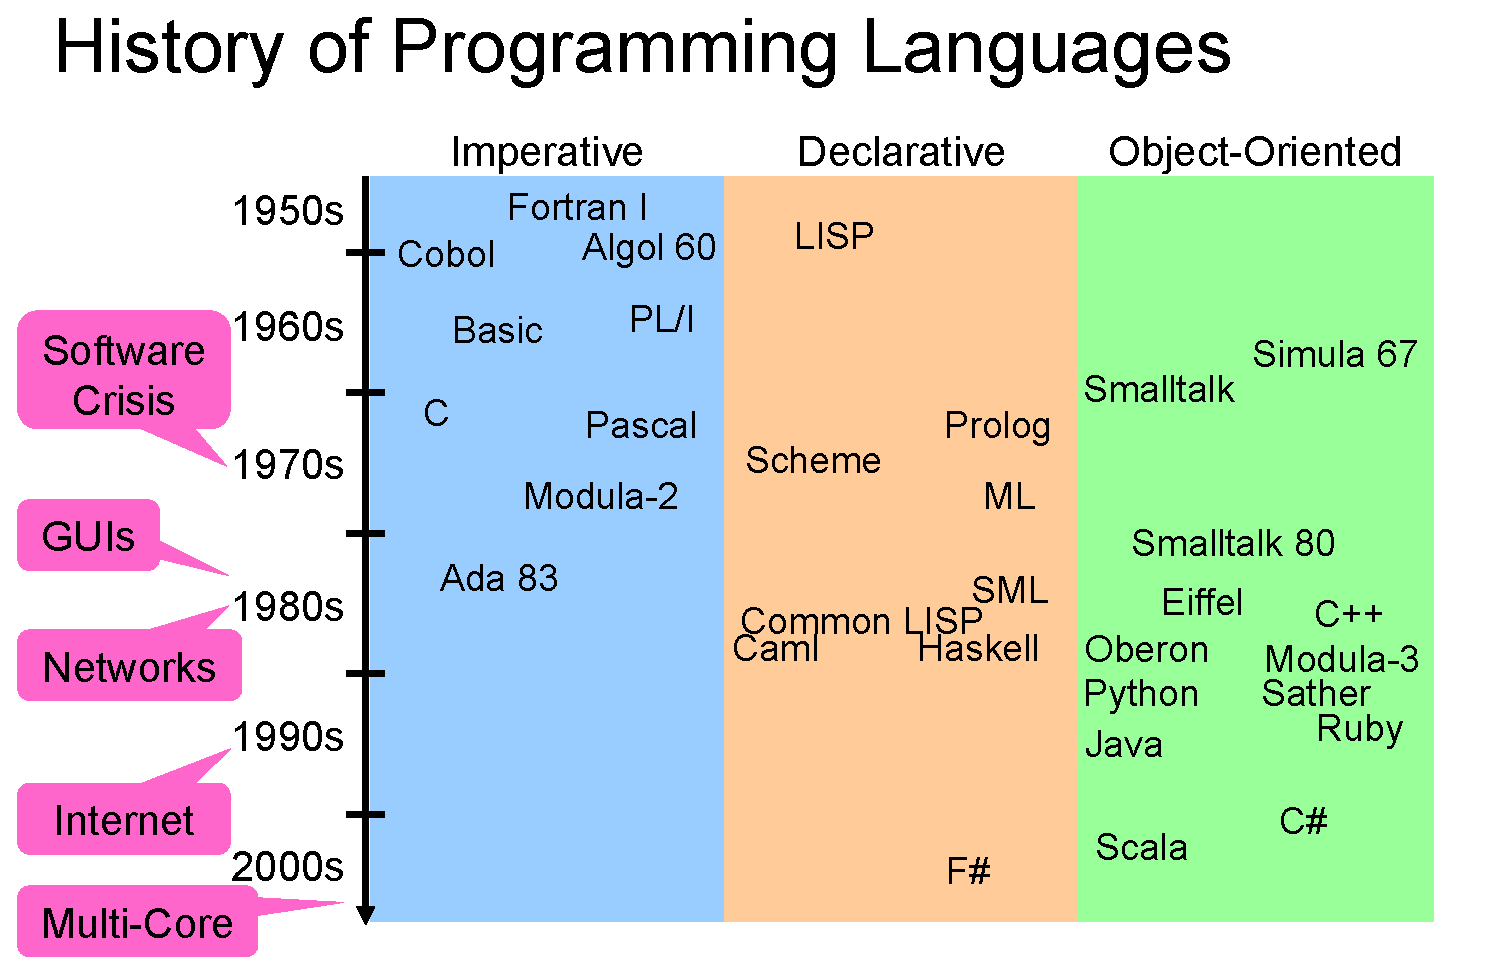
\includegraphics[width=0.7\textwidth]{img/01_programming_languages}
      \caption{History of Programming Languages}

\end{figure}

Which forced a rethinking process.
\begin{figure}[h!]
  \centering
    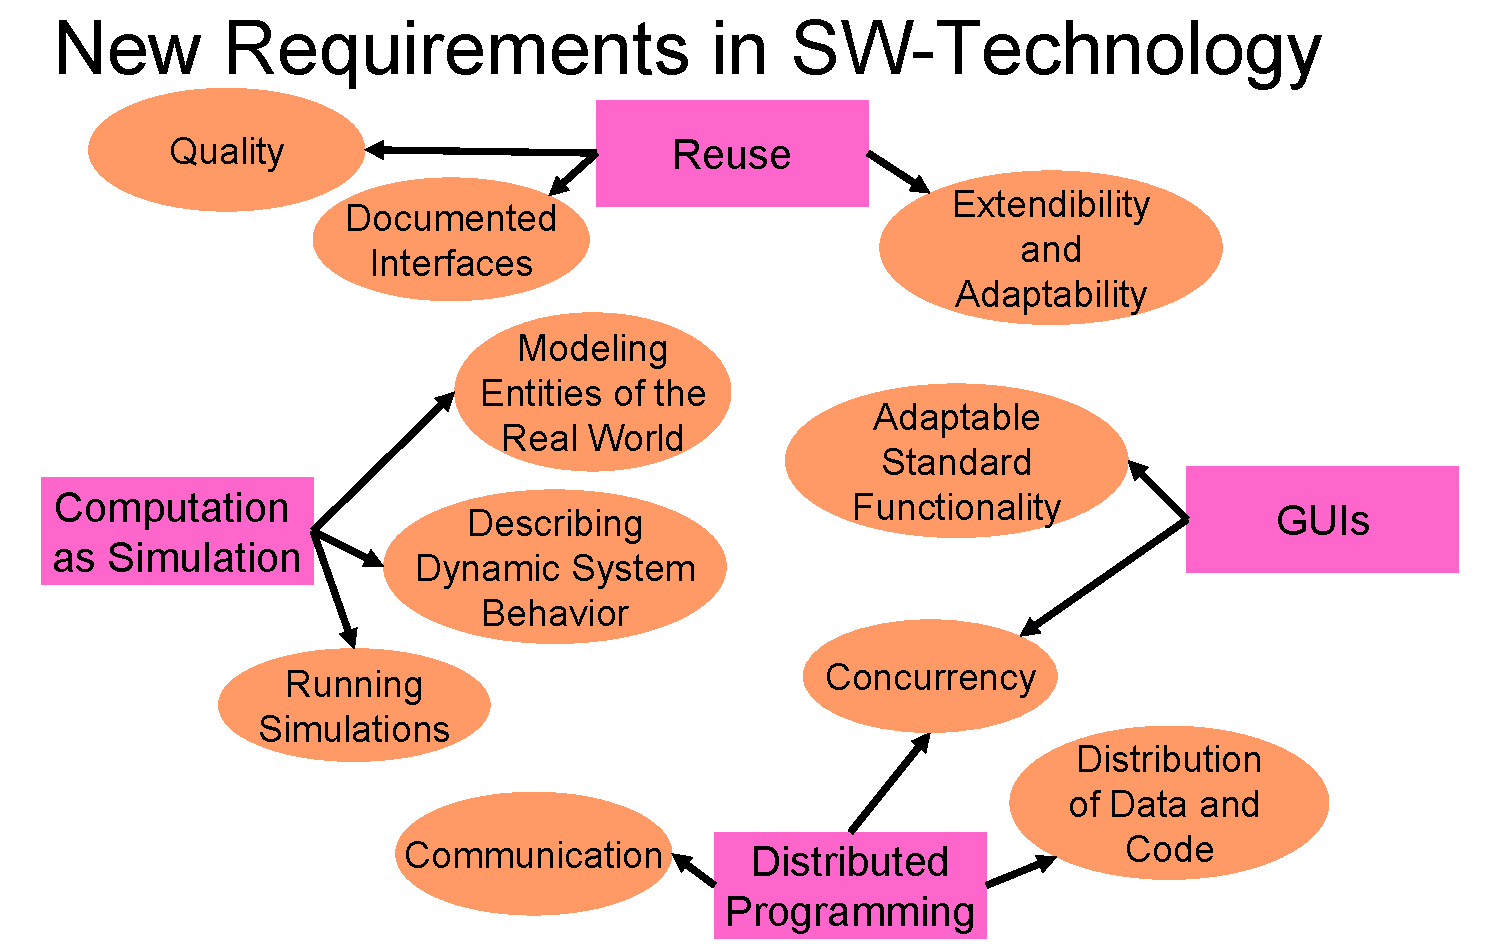
\includegraphics[width=0.7\textwidth]{img/01_new_requirements}
      \caption{New Requirements in Software Technology}
\end{figure}

\subsection{Study: Reusing Imperative Programs}
We try to model a University Administration System:
\begin{itemize}
 \item Which models students and professors
 \item Stores one record for each student and each professor in a repository
 \item A procedure printAll prints all records in the repository
\end{itemize}

\lstset{language=C}
\begin{lstlisting}[caption=Implementation in C]
typedef struct {
  char *name;
  char *room;
  char *institute;
} Professor;

typedef struct {
  char *name;
  int  regnum;
} Student;

void printStudent(Student *s) {...}
void printProf(Professor *p) {...}

typedef struct {
  enum { STU,PROF } kind;
  union {
    Student *s;
    Professor *p;
  } u;
} Person;

typedef Person **List;

void printAll( List l ) {
  int i;
  for ( i=0; l[ i ] != NULL; i++ )
    switch ( l[ i ] -> kind ) {
    case STU:
      printStudent( l[ i ] -> u.s );
      break;
    case PROF:
      printProf( l[ i ] -> u.p );
      break;
  }
}
\end{lstlisting}

\paragraph{Extending the System} in order to extend the system with assistants on has to:
\begin{itemize}
 \item Add a record and print function for the assistants
 \item Reuse old code for repository and printing
\end{itemize}

\begin{lstlisting}[caption=Extending the system]
// Student and Professor structs
typedef struct {
  char *name;
  char PhD_student; /* ‘y‘, ‘n‘ */
} Assistant;

// Student and Professor print code
void printAssi(Assistant *a) {...}

// Change the Person struct
typedef struct {
  enum { STU,PROF,ASSI } kind;
  union {
    Student *s;
    Professor *p;
    Assistant *a;
  } u;
} Person;

// Change the printAll function
void printAll( List l ) {
  int i;
  for ( i=0; l[ i ] != NULL; i++ )
    switch ( l[ i ] -> kind ) {
    case STU:
      printStudent( l[ i ] -> u.s );
      break;
    case PROF:
      printProf( l[ i ] -> u.p );
      break;
    case ASSI:
      printAssi( l[ i ] -> u.a );
      break;
  }
}
\end{lstlisting}

\subsection{Reuse in Imperative Languages}
\begin{itemize}
 \item Imperative languages don't have an explicit language support for extension and adaption
 \item Adaption usually requires modification reused code
 \item Code adaption requires \textbf{Copy-and-paste reuse} which leads to
  \begin{itemize}
   \item Code duplication
   \item Is difficult to maintain
   \item Is \emph{Error-prone}
  \end{itemize}

\end{itemize}

\subsection{Core Requirements}
All of this leads to these core requirements for object oriented programming languages:
\begin{figure}[h!]
  \centering
    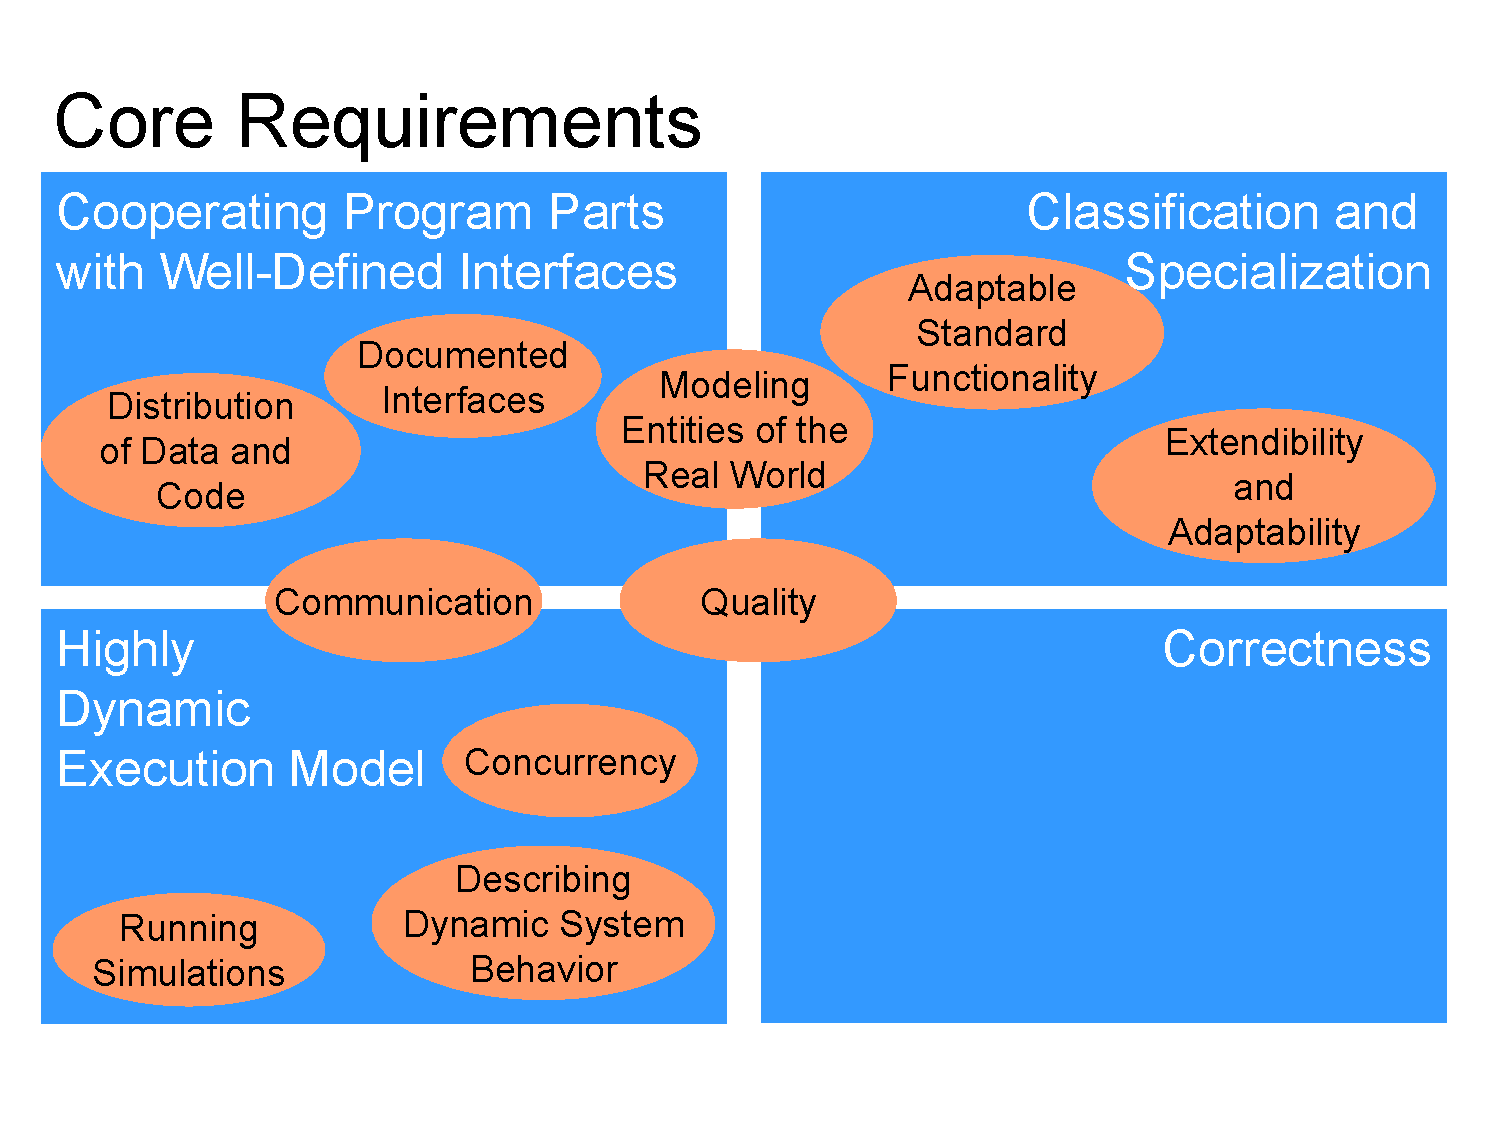
\includegraphics[width=0.7\textwidth]{img/01_core_requirements}
      \caption{Core Requirements in Software Technology}
\end{figure}

\section{Core Concepts}
\begin{shadequote}
The basic philosophy underlying object-oriented
programming is to make the programs as far as
possible reflect that part of the reality they are going
to treat. It is then often easier to understand and to
get an overview of what is described in programs.
The reason is that human beings from the outset are
used to and trained in the perception of what is going
on in the real world. The closer it is possible to use
this way of thinking in programming, the easier it is to
write and understand programs.\par\emph{Object-oriented Programming in the BETA Programming Language}
\end{shadequote}
\subsection{The Object Model}
\begin{itemize}
 \item A software system is a set of cooperating object
 \item Objects have state and processing ability
 \item Objects exchange messages
\end{itemize}
\begin{figure}[H]
  \centering
    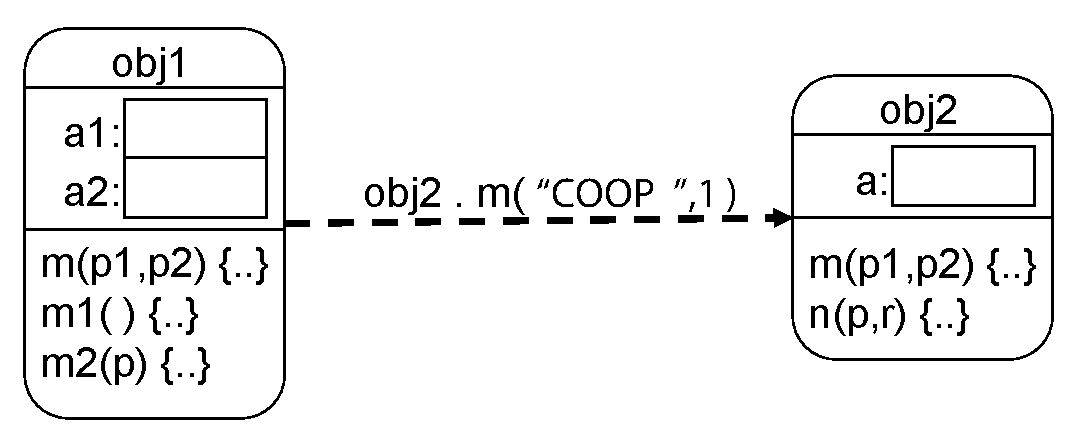
\includegraphics[width=0.5\textwidth]{img/01_object_model}
      \caption{The object model}
\end{figure}
\subsubsection{Characteristics of Objects}
\begin{itemize}
 \item State
 \item Identity
 \item Lifecycle
 \item Location
 \item Behavior
\end{itemize}
Compared to imperative programming, 
\begin{itemize}
 \item Objects lead to a \emph{different program structure}
 \item Objects lead to a \emph{different execution model}
\end{itemize}

\subsection{Interfaces and Encapsulation} 
\begin{itemize}
 \item Objects have \textbf{well-defined interfaces}
  \begin{itemize}
   \item Publicly accessible fields
   \item Publicly accessible methods
  \end{itemize}
 \item \text{Implementation is hidden} behind interface
  \begin{itemize}
   \item Encapsulation
   \item Information hiding
  \end{itemize}
 \item Interfaces are the basis for \textbf{describing behavior}
\end{itemize}

\subsection{Classification and Polymorphism}
\begin{itemize}
 \item \textbf{Classification}: Is a hierarchical structuring of objects
 \item Objects belong to different classes simultaneously
 \item \textbf{Substitution principle}: Subtype objects can be used wherever supertype objects are expected.
\end{itemize}

\begin{definition}[Classification]
Classifying is a general technique to hierarchically
structure knowledge about concepts, items, and
their properties.\\
The result is called classification.
\end{definition}

\paragraph{Characteristics of Classifications} We can classify objects or fields:
\begin{itemize}
 \item Classifications can be \emph{trees} or \emph{DAGs}
 \item Classifications of objects form \emph{``is-a'' relation}.
 \item Classes can be \emph{abstract} or \emph{concrete}.
\end{itemize}
\begin{definition}[Substitution principle]
Objects of subtypes can be used wherever objects are expected.
\end{definition}

\subsection{Polymorphism}
\begin{shadequote}
The quality of being able to assume different forms.\par\emph{Merriam-Webster Dictionary}
\end{shadequote}

\begin{definition}A program part is polymorphic if it can be used for objects of several types.
\end{definition}

\paragraph{Subtype Polymorphism} is a direct consequence of the substitution principle.
\begin{itemize}
 \item Program parts working with supertype objects work as well with subtype objects
 \item Example: \lstinline{ printAll } can print objects of class Person, Student, Professor, etc.
\end{itemize}
\subsection{Other forms of polymorphism}
\begin{description}
 \item[Parametric Polymorphism] Generic types
  \begin{itemize}
   \item Uses \emph{type parameters}
   \item One implementation can be used for different types
   \item \emph{Type mismatches can be detected at compile time}
  \end{itemize}
  \lstset{language=Java}
  \begin{lstlisting}
  class List<G> {
    G[ ] elems;
    void append( G p ) { ... }
  }
  
  List<String> myList;
  myList = new List<String>( );
  myList.append( “String” );
  \end{lstlisting}
 \item[Ad-hoc Polymorphism] Method overloading
  \begin{itemize}
   \item Allows several methods with the \emph{same name but different arguments}
   \item Also called \emph{overloading}
   \item No semantic concept: Can be modeled by \emph{renaming}
  \end{itemize}
  \begin{lstlisting}
  class Any {
    void foo( Polar p ) { ... }
    void foo( Coord c ) { ... }
  }
  x.foo( new Coord( 5, 10 ) );
  x.foo( new Polar( 5, 10 ) );
  \end{lstlisting}
\end{description}

\subsection{Specialization}
\begin{definition}
 Adding specific properties to an object or refining a concept by adding further characteristics.
\end{definition}




\section{Cache Coherence}
Processor speed improves (approx.) 60\% per year:
\begin{itemize}
	\item until 2005 mainly by increasing the clock rate,
	\item after 2005 by increasing the number of cores.
\end{itemize}
The memory speed however only improves by (approx.) 10\% per year. Which results in a widening performance gap.
 
Caching may result in multiple copies for a memory location in multiple caches. Cache coherence manages the existence of multiple copies. 
\emph{Requirements}: 
\begin{itemize}
	\item Write propagation: Writes are eventually visible to all processors
	\item Write serialisation: Every processor should see the writes to the same location in the same order.
\end{itemize}

\begin{description}
	\item[Concerns] $\text{}$
		\begin{itemize}
			\item Performance
			\item Implementation cost
			\item Correctness
		\end{itemize}
	\item[Issues] $\text{}$
		\begin{itemize}
			\item Detection (when is it necessary for the cache controller to become active)
			\item Enforcement (how the coherence is established)
			\item Precision of block-sharing information
			\item Block size
		\end{itemize}
	\item[Mechanisms] $\text{}$
		\begin{description}
			\item[Snooping-based cache coherence] $\text{}$
				\begin{itemize}
					\item Shared bus or network
					\item Cache controller "snoops" (observes) bus transactions
					\item Cache controller aware of state of the cache's data
				\end{itemize}

			\item[Directory-based cache coherence] Record (in memory) information necessary to maintain coherence
		\end{description}

\end{description}

\subsection{Problems}
\begin{enumerate}
	\item Stale values
		\begin{itemize}
			\item $CPU_1$ uses stale value that has already been modified by $CPU_0$
			\item \emph{Solution} 
				\begin{itemize}
					\item Don't allow this to happen
					\item Invalidate all copies before allowing a write to proceed
				\end{itemize}
		\end{itemize}
	\item Loosing result of a write
		\begin{itemize}
			\item An incorrect write-back order of modified cache lines applies the writebacks in an order different from the order of the write operations
			\item \emph{Solution}> Disallow more than one modified copz
		\end{itemize}
\end{enumerate}

\subsection{Protocol Approaches}
\begin{description}
	\item[Invalidation-based] $\text{}$
		\begin{itemize}
			\item All coherency-related traffic broadcast to all CPUs
			\item Each processor snoops traffic and reacts accordingly
				\begin{itemize}
					\item Invalidate lines written to by antother CPU
					\item Signal sharing for cache lines currently in cache
				\end{itemize}
			\item Straightforward solution for bus-based systems
			\item Suited for small-scale systems
			\item Comparison:
				\begin{itemize}
					\item Only write misses hit the bus (suited for write-back caches)
					\item Subsequent writes to the cache-line are write-hits
					\item Good for multiple writes to the same cache line by the same CPU
				\end{itemize}

		\end{itemize}
	\item[Update-based] $\text{}$
		\begin{itemize}
			\item Uses central directory for cache line ownershop
			\item Write operation updates copies in other caches
				\begin{itemize}
					\item Can update all other CPUs at once (less bus traffic)
					\item But: Multiple writes cause multiple updates (more bus traffic)
				\end{itemize}
			\item Suited for large-scale systems
			\item Comparison:
				\begin{itemize}
					\item All sharers of a cache line continue to hit in the cache after a write by one cache.
						\emph{Assumption}: There are more accesses until this line must be evicted for other reasons.
					\item Well-suited for producer-consumer pattern
					\item Risks wasting bandwidth
				\end{itemize}

		\end{itemize}
\end{description}

\subsection{MESI Protocol}
Each cache line is in one of $4$ states>
\begin{description}
	\item[Modified (M)] $\text{}$
		\begin{itemize}
			\item No copies in other caches, local copy has been modified
			\item Memory is stale
		\end{itemize}
	\item[Exclusive (E)]
		\begin{itemize}
			\item No copies of other caches
			\item Memory is up to date
		\end{itemize}
	\item[Shared]
		\begin{itemize}
			\item Unmodified copies \emph{may} exist in other caches
			\item Memorz is up to date
		\end{itemize}

	\item[Invalid (I)] not in cache
\end{description}



\end{document}
